\section{Auswertung}
\label{sec:Auswertung}
<<<<<<< HEAD

Bevor die spezifische Wärmekapazität der Proben untersucht werden kann, muss zunächst das Produkt 
aus spezifische Wärmekapazität $c_g$ und Masse $m_g$ des Dewargefäßes bestimmt werden. 
Dieses ergibt sich, wenn die abgegebene Wärme 
\begin{equation}
    Q_{erhitzt} = c_{W} m_{W,heiss} (T_{erhitzt}-T_{vermischt})
\end{equation}
des erhitzten Wassers mit der aufgenommenen Wärme 
\begin{equation}
    Q_{kalt} + Q_{Wand} = (c_{W}  m_{W,kalt} + c_g m_g) (T_{vermischt} - T_{kalt})
\end{equation}
des kalten Wassers und der Wand des Dewargefäßes gleichgesetzt und nach $c_g m_g$ aufgelöst wird.
Werden zur Berechnung die in Tabelle \ref{tab:1} aufgeführten Werte verwendet und der Wert 
der spezifischen Wärmekapazität des Wassers als $c_{W} = 4,18\, \si{\joule\per\kelvin} $ (ZITAT),
ergibt sich 
\begin{equation}
    c_g m_g = 399,35\, \si{\joule\per\kelvin}
\end{equation}
\noindent als gesuchter Wert.

\begin{table}[h]
\normalsize

\centering
\sisetup{table-format=4.0}
\begin{tabular}{c c c c c}
\toprule
        $m_{Wasser,1} \,/\, \si{\gram}$ &$ m_{Wasser,2} \,/\, \si{\gram}$ & $T_{kalt} \,/\, \si{\kelvin} $& $T_{heiss} \,/\, \si{\kelvin} $& $T_{vermischt} \,/\, \si{\kelvin} $\\
        \midrule
        287,58 & 273,24‬ & 294,95 & 353,15 & 320,45 \\

\bottomrule

\end{tabular}

\caption{Messwerte zur Bestimmung von $c_g m_g$}
\label{tab:1}
\end{table}
\noindent
Nun kann mithilfe dieser Größe die spezifische Wärmekapazität der einzelnen Proben untersucht werden.





\subsection{Bestimmung der Wärmekapazitäten}

\subsubsection{Allgemein}

Um die spezifische Wärmekapazität einer Probe zu erhalten, müssen die beiden Gleichungen (VERWEIS)
gleichgesetzt und nach $c_{Probe}$ umgestellt werden. In die dabei erhaltene Gleichung
\begin{equation}
    c_{Probe} = \frac{(c_{W} m_{W} + c_{g} m_{g}) (T_{vermischt}-T_{W}) }{m_{Probe} (T_{Probe}-T_{vermischt})}
    \label{eq:euler}
\end{equation}
\noindent können die aufgenommenen Messwerte eingesetzt werden. Weiterhin soll die Formel
\begin{equation}
    \bar{x}=\frac{1}{N}\sum_{i=1}^N x_i
    \label{eq:mittelwert}
\end{equation}
\noindent zur Berechnung des Mittelwerts und
\begin{equation}
     \Delta\bar{x}=\sqrt{\frac{1}{N(N-1)}\sum_{i=1}^N (x_i-\bar{x})^2}
     \label{eq:std}
 \end{equation}
\noindent zur Berechnung des Standardfehler des Mittelwerts verwendet werden.



\subsubsection{Kupfer}

Für die drei Messungen ergeben sich mithilfe der in Tabelle \ref{tab:2} aufgeführten Werte 
und der Gleichung \ref{eq:euler} die Werte 
\begin{align}
    c_{Cu,1} = 0,44\, \si{\joule\per\gram\per\kelvin} \nonumber \\
    c_{Cu,2} = 0,42\, \si{\joule\per\gram\per\kelvin} \nonumber \\
    c_{Cu,3} = 0,42\, \si{\joule\per\gram\per\kelvin} \\
    \label{align:wertekupfer}
\end{align}
\noindent für die spezifische Wärmekapazität von Kupfer. Weiterhin ergibt sich über die 
Gleichungen \ref{eq:mittelwert} und \ref{eq:std} der 
Wert $c_{Cu} = (0,427 \pm 0,006)\, \si{\joule\per\kelvin}$.




\begin{table}[h]
\normalsize

\centering
\sisetup{table-format=4.0}
\begin{tabular}{c c c c c c}
\toprule
        Messung & $m_{Wasser} \,/\, \si{\gram}$ & $ m_{Probe} \,/\, \si{\gram}$ & $T_{Wasser} \,/\, \si{\kelvin} $& $T_{Probe} \,/\, \si{\kelvin} $& $T_{vermischt} \,/\, \si{\kelvin} $\\
        \midrule
        1 & 557,39 & 235,46‬ & 295,85 & 358,75 & 298,15 \\
        2 & 564,51 & 235,46‬ & 294,85 & 358,75 & 297,05 \\
        3 & 491,41 & 235,46‬ & 294,45 & 358,85 & 296,95 \\

\bottomrule

\end{tabular}

\caption{Messwerte zur Bestimmung von $c_{Cu}$}
\label{tab:2}
\end{table}



\subsubsection{Aluminium}

Für die drei Messungen ergeben sich mithilfe der in Tabelle \ref{tab:3} aufgeführten Werte 
und der Gleichung \ref{eq:euler} die Werte 
\begin{align}
    c_{Al,1} = 0,90\, \si{\joule\per\gram\per\kelvin} \nonumber \\
    c_{Al,2} = 0,98\, \si{\joule\per\gram\per\kelvin} \nonumber \\
    c_{Al,3} = 0,87\, \si{\joule\per\gram\per\kelvin} \nonumber \\
    \label{align:wertealuminium}
\end{align}
\noindent für die spezifische Wärmekapazität von Aluminium. Weiterhin ergibt sich über die 
Gleichungen \ref{eq:mittelwert} und \ref{eq:std} der 
Wert $c_{Al} = (0,917 \pm 0,027)\, \si{\joule\per\kelvin}$.


\begin{table}[h]
\normalsize

\centering
\sisetup{table-format=4.0}
\begin{tabular}{c c c c c c}
\toprule
        Messung & $m_{Wasser} \,/\, \si{\gram}$ & $ m_{Probe} \,/\, \si{\gram}$ & $T_{Wasser} \,/\, \si{\kelvin} $& $T_{Probe} \,/\, \si{\kelvin} $& $T_{vermischt} \,/\, \si{\kelvin} $\\
        \midrule
        1 & 565,68 & 111,27‬ & 295,35 & 358,55 & 297,55 \\
        2 & 573,10 & 111,27‬ & 294,95 & 358,65 & 297,35 \\
        3 & 528,57 & 111,27‬ & 294,75 & 358,75 & 297,05 \\

\bottomrule

\end{tabular}

\caption{Messwerte zur Bestimmung von $c_{Al}$}
\label{tab:3}
\end{table}




\subsubsection{Graphit}

Für die drei Messungen ergeben sich mithilfe der in Tabelle \ref{tab:4} aufgeführten Werte und der Gleichung
\ref{eq:euler} die Werte 
\begin{align}
    c_{Graphit,1} = 0,690\, \si{\joule\per\gram\per\kelvin}  \\
    \label{align:wertegraphit}
\end{align}
\noindent für die spezifische Wärmekapazität von Graphit.


\begin{table}[h]
\normalsize

\centering
\sisetup{table-format=4.0}
\begin{tabular}{c c c c c c}
\toprule
        Messung & $m_{Wasser} \,/\, \si{\gram}$ & $ m_{Probe} \,/\, \si{\gram}$ & $T_{Wasser} \,/\, \si{\kelvin} $& $T_{Probe} \,/\, \si{\kelvin} $& $T_{vermischt} \,/\, \si{\kelvin} $\\
        \midrule
        1 & 534,30 & 105,85‬ & 294,85 & 358,25 & 296,55 \\

\bottomrule

\end{tabular}

\caption{Messwerte zur Bestimmung von $c_{Graphit}$}
\label{tab:4}
\end{table}


\subsection{Berechnung der Molwärme}
 
\subsubsection{Kupferprobe}
Mithilfe der Gleichungen \ref{eq:zusammenhangcvcp} und
\begin{equation}
    C_{P} = M c_K,
\end{equation}
\noindent
den zuvor berechneten Werten für die spezifischen
Wärmekapazitäten der einzelnen Proben, den gemessenen Temperaturen $T_{vermischt}$ und den 
vorgegebenen Werten für $\alpha$ und $\kappa$ \cite{sample}, 
lassen sich nun die Molwärmen berechnen. Mit den Werten
\ref{align:wertekupfer} ergeben sich somit 
\begin{align}
    C_{V,Cu,1} = 27,21\, \si{\joule\per\mole\per\kelvin} \nonumber \\
    C_{V,Cu,2} = 25,94\, \si{\joule\per\mole\per\kelvin} \nonumber \\
    C_{V,Cu,3} = 25,94\, \si{\joule\per\mole\per\kelvin}, \\
    \label{align:wertekupfer}
\end{align}
\noindent 
welche nun über Gleichung \ref{eq:mittelwert} und \ref{eq:std} gemittelt werden können. Folglich ergibt sich
\begin{equation}
    C_{V,Cu} = 26,36 \pm 0,43\, \si{\joule\per\mole\per\kelvin}
\end{equation}
als Molwärme $C_{V,Cu}$ für Kupfer.




\subsubsection{Aluminiumprobe}
Über ein analoges Vorgehen, wie bei Kupferprobe lässt sich auch hier die Molwärme 
berechnen. Mit dem Wert \ref{align:wertealuminium} ergeben sich somit 
\begin{align}
    C_{V,Al,1} = 23,19\, \si{\joule\per\mole\per\kelvin} \nonumber \\
    C_{V,Al,2} = 25,35\, \si{\joule\per\mole\per\kelvin} \nonumber \\
    C_{V,Al,3} = 22,38\, \si{\joule\per\mole\per\kelvin}, \\
    \label{align:wertealuminium}
\end{align}
\noindent 
welche nun über Gleichung \ref{eq:mittelwert} und \ref{eq:std} gemittelt werden können. Folglich ergibt sich
\begin{equation}
    C_{V,Al} = 23,64 \pm 0,80\, \si{\joule\per\mole\per\kelvin}
\end{equation}
als Molwärme $C_{V,Al}$ für Aluminium.





\subsubsection{Graphitprobe}
Über ein analoges Vorgehen, wie bei Kupferprobe lässt sich auch hier die Molwärme berechnen. Mit dem Wert
\ref{align:wertegraphit} ergebt sich somit 
\begin{equation}
    C_{V,Graphit} = 8,25 \pm 0,69\, \si{\joule\per\mole\per\kelvin}
\end{equation}
als Molwärme für Graphit.



||||||| merged common ancestors

\begin{figure}
  \centering
  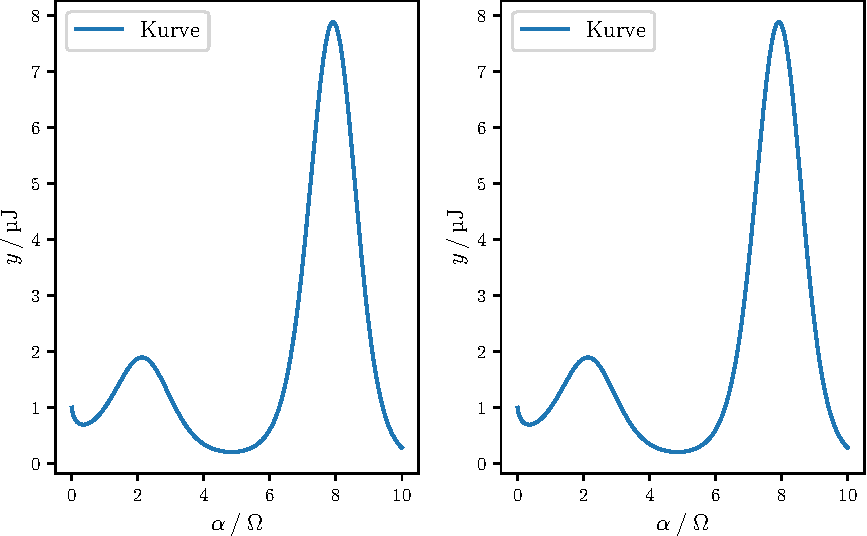
\includegraphics{plot.pdf}
  \caption{Plot.}
  \label{fig:plot}
\end{figure}


Siehe \autoref{fig:plot}!
=======
>>>>>>> refs/remotes/origin/master
